\section{Introduction}

\begin{frame}
	\frametitle{Challenging Problem}
	
	\begin{center}
		\begin{tikzpicture}
			\node at (0,0) [draw=white,ultra thick,inner sep=0pt]
			{
				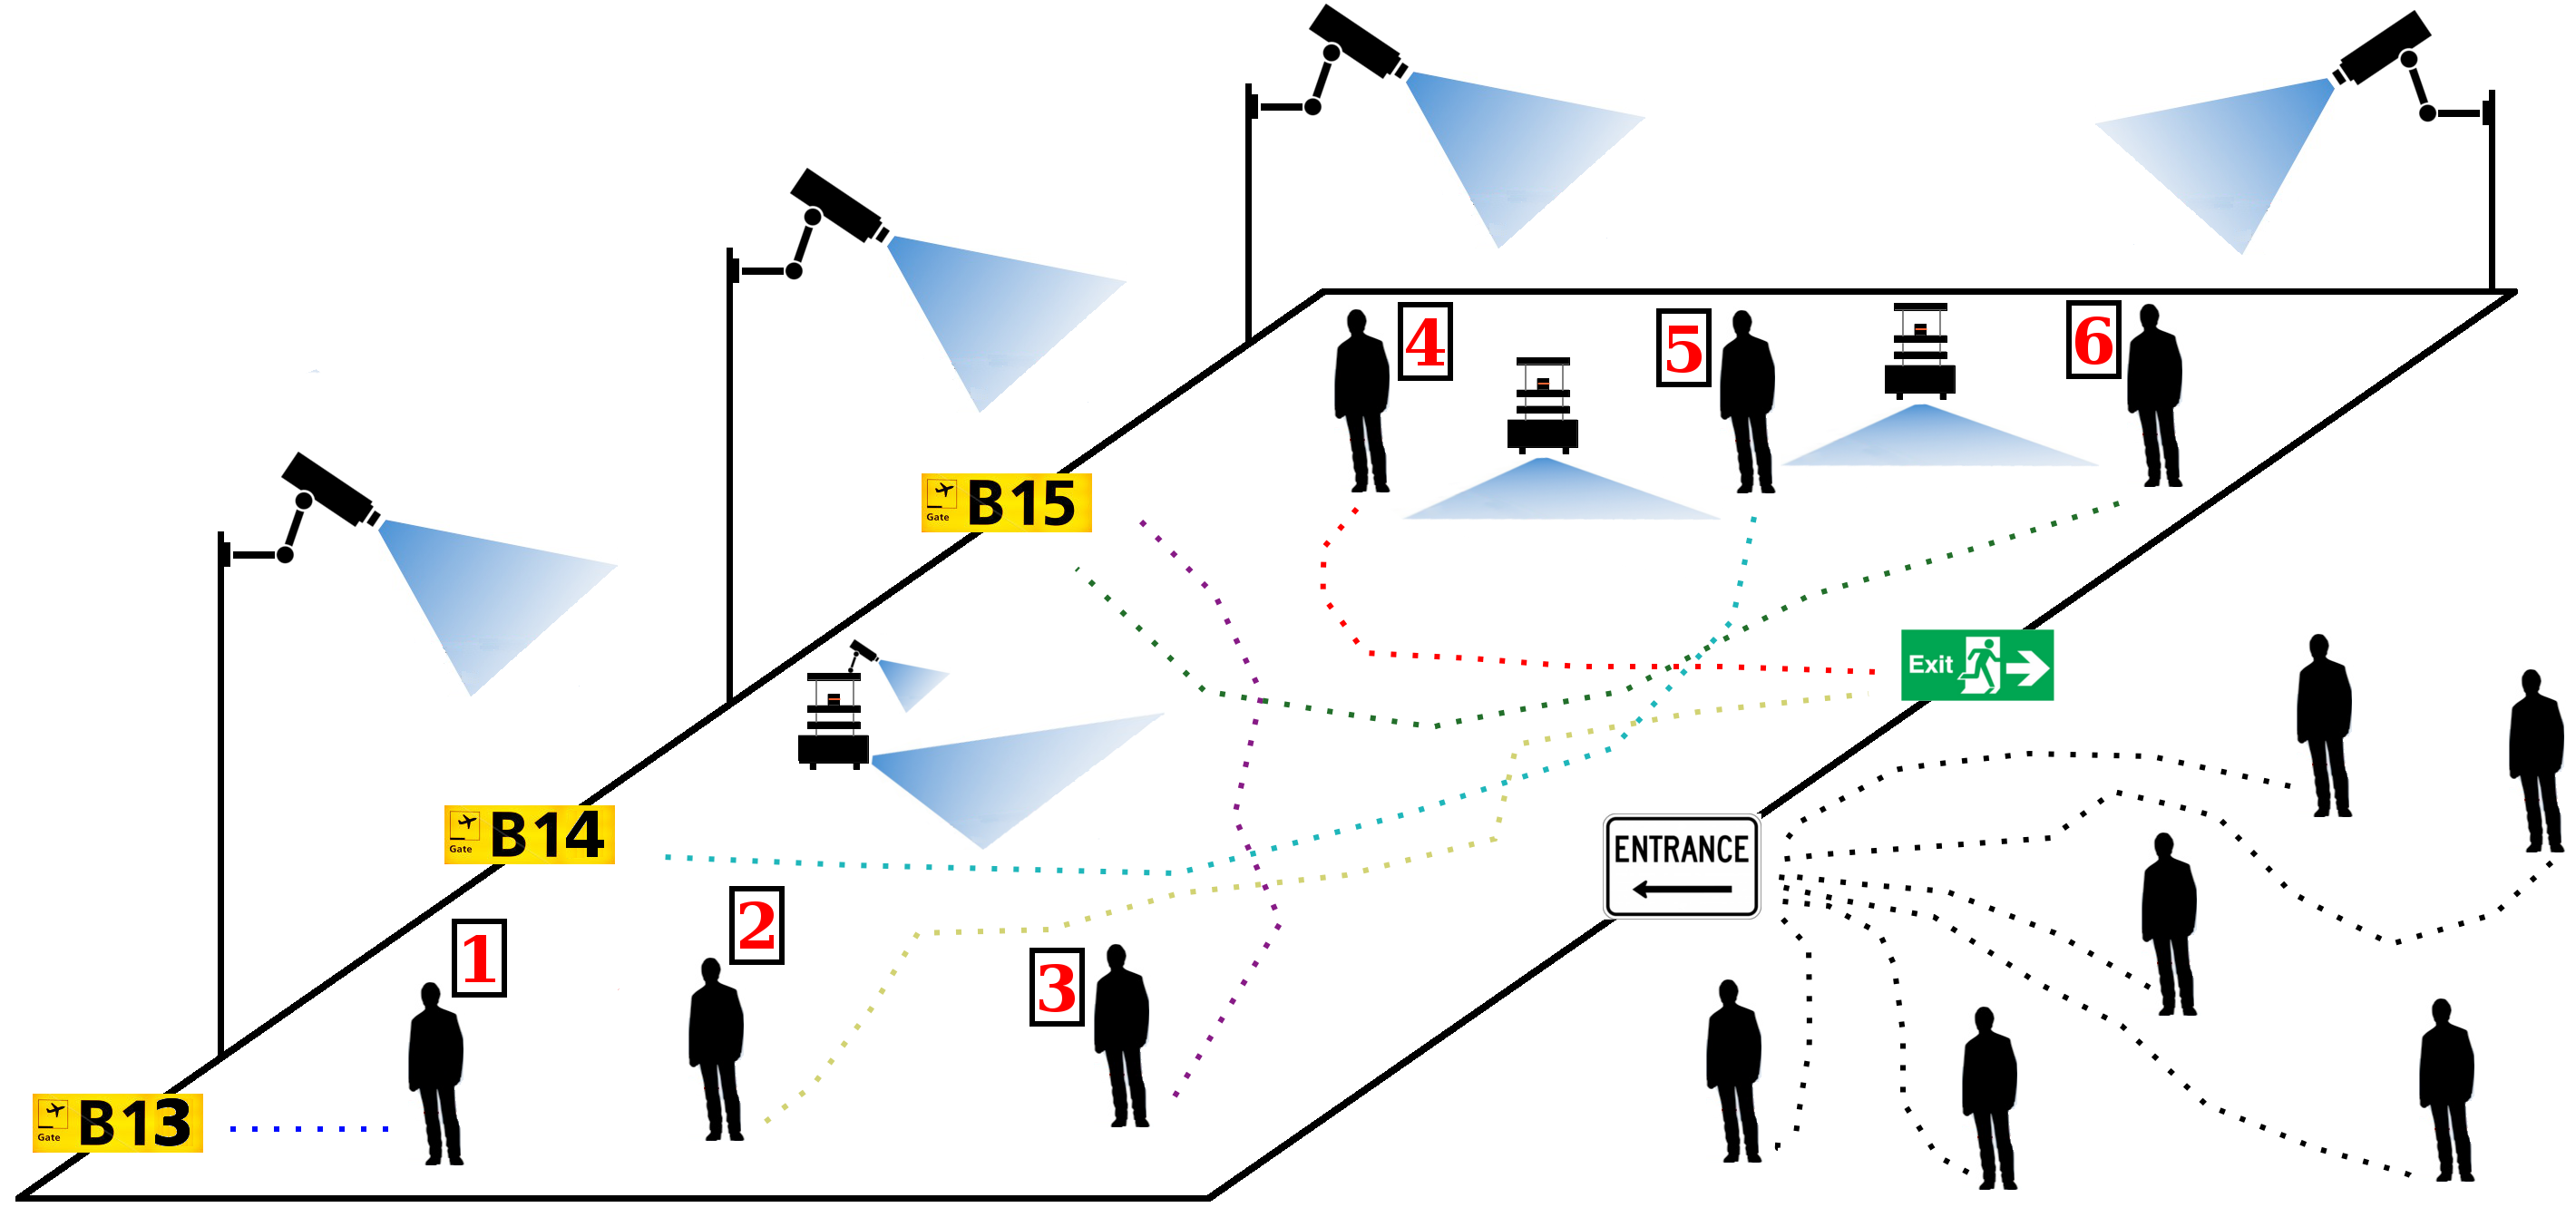
\includegraphics[scale=0.12]{Figures/Problem.png}
			};
		\end{tikzpicture}
	\end{center}
\end{frame}

\begin{frame}
	\frametitle{Related Work}
	\framesubtitle{Human Activity Classification and Activity Recognition}
	
	\vspace{0.4cm}
	
	\begin{columns}[T]
		\column{.55\textwidth}
		
		\vspace{0.2cm}
		
		\begin{itemize}
			\item \textbf{Nascimento et al. [1]:} recognise pedestrian trajectories in
				  video sequences, in a surveillance context
			
			\vspace{1.2cm}
			
			\item \textbf{Veloso et al. [2]:} discriminatively trained Conditional Random
				  Fields for activity recognition
		\end{itemize}
		
		\column{.5\textwidth}
		
		\centering
		\begin{tikzpicture}
			\node at (1.42,0) [draw=black,ultra thick,inner sep=0pt]
			{
				\includegraphics[height=2.2cm]{Figures/Nascimento-1}
			};
			\node at (-1.42,0) [draw=black,ultra thick,inner sep=0pt]
			{
				\includegraphics[height=2.2cm]{Figures/Nascimento-2}
			};
			\node at (0,-2.8) [draw=black,ultra thick,inner sep=0pt]
			{
				\includegraphics[width=5cm]{Figures/Veloso}
			};
		\end{tikzpicture}
	\end{columns}
	
	\vspace{0.37cm}
	
	\tiny
	
	[1] J. C. Nascimento et al., ``Trajectory classification using switched dynamical
		hidden markov models,'' Image Processing, 2010
	
	\vspace{-0.17cm}
	
	[2] D. L. Vail, M. M. Veloso, J. D. Lafferty, ``Conditional random fields for activity
		recognition,'' AAMAS, 2007
\end{frame}

\begin{frame}
	\frametitle{Related Work}
	\framesubtitle{Activity Forecasting through Semantic Mapping}
	
	\vspace{0.33cm}
	
	\large
	
	\textbf{Ziebart et al. [3]} proposed a method for activity forecasting by combining:
	
	\begin{itemize}
		\item Semantic scene understanding
		\vspace{0.05cm}
		\item Inverse Optimal Control
	\end{itemize}
	
	\vspace{-0.2cm}
	
	\begin{center}
		\begin{tikzpicture}
			\node at (0,0) [draw=white,ultra thick,inner sep=0pt]
			{
				\includegraphics[scale=0.19]{Figures/ActivityForecasting.png}
			};
		\end{tikzpicture}
	\end{center}
	
	\vspace{-0.3cm}
	
	\tiny
	
	[3] K. Kitani, B. D. Ziebart, J. A. Bagnell, M. Hebert, ``Activity Forecasting'', ECCV,
		2012
\end{frame}

\begin{frame}
	\frametitle{Advantages/Disadvantages}
	
	\Large
	
	\vspace{0.6cm}
	
	\underline{\textbf{Advantages}} \\
	
	\vspace{0.2cm}
	
	\begin{itemize}
		\item knowledge transfer by using physical scene features
		\item accurate and robust destination forecasting
	\end{itemize}
	
	\vspace{0.2cm}
	
	\underline{\textbf{Disadvantages}} \\
	
	\vspace{0.19cm}
	
	\begin{itemize}
		\item prior knowledge of potential goals
		\item space of possible motions is explicitly parametrised
		\item applicability in dynamic environments? \\
			  \vspace{-0.2cm}
			  \begin{tabbing}
				  \hspace{0.3cm}
				  \large
				  $ \leadsto $ \emph{rescue or rapidly changing construction environment}
			  \end{tabbing}
	\end{itemize}
\end{frame}
